\chapter{Konzeption} % Das würde eigentlich 'Konzeption' heißen aber Tichy wirkt stark in mir

hier kurz beschreiben, was so grob abgeht, also was wir so machen wollen und was für netze wir vergleichen wollen,
um das beste zu finden

\section{Datensatz für Fahrradwege}


\section{Pre-Processing}

zerschneiden - warum 512x512 und nicht 256x256, rauswerfen. 

train images: 7738
val images: 672    <- 8\% der test bilder, 6,6\% aller
sum:        8410
test:       1771  <- 17,5\% aller Bilder 
sum:        10181 <- nur 17,7\% aller möglichen bilder

eigentlich $143 Bilder * round_up(10_000 / 512)^2 = 143 * 20^2 = 57200$

Verhältnis weiß : schwarz < 1 : 100, dann wird bild übersprungen

jede der folgenden augmentationen wird in jeweils ihrer Domäne random gleichzeitig applied.
Zudem wird für jede Batch geshuffled, die Einteilung in train und test ist ebenfalls geshuffled 
% augmentation = {
% 	"rotation_range": 90,
% 	"width_shift_range": 0.1,
% 	"height_shift_range": 0.1,
% 	"fill_mode": "constant",
% 	"cval": 0,
% 	"horizontal_flip": "True",
% 	"vertical_flip": "True",
% 	"validation_split": 0.08
% }

\subsection{Daten-Augmentation}

\section{Architektur} \label{sec:architecture}

Im Folgenden werden die untersuchten Architekturen genauer beschrieben und ebenfalls begründet, 
warum die jeweiligen architektonischen Entscheidungen getroffen wurden. \\
In \autoref{sec:state-of-the-art-roads} wurde ausführlich der Stand der Technik und Wissenschaft 
im Bereich der Straßenerkennung und -extraktion mittels Computer-Vision-Modellen beschrieben. 
Aufgrund der Ähnlichkeit der Problemdomäne lässt sich vermuten, dass ähnliche Verfahren wie 
zum Erkennen von Straßen auch für das Erkennen von Fahrradwegen nützlich sein könnten. 
Die Problemdomänen sind ähnlich, da Fahrradwege auch Straßen sind und eben jene Eigenschaften, 
wie große Klassenimbalance zwischen Fahrradweg und Hintergrund, Beschattung durch andere Objekte,
Verdeckung durch z.B. Bäume und ähnliche Annotationsfehler   
teilen. Schwierigkeit hier wird sein, Fahrradwege von Straßen zu unterscheiden. \\
Die Radwege sollen, wie Straßen auch, mittels Image-Semantic-Segmentation von einem Computer-Vision-Modell 
markiert werden. Andere Klassifizierungsarten, wie die in \autoref{sec:aufgabenkategorien} beschriebene 
Objektdetektion würde zu grobe Bounding-Boxes um schräg verlaufende Radwege legen, sodass im Prinzip 
eine Straße markiert werden würde, die zwar ein Radweg hat, aber nicht klar wäre, wo dieser verläuft, 
bzw. ob ein Radweg in beide Richtungen existiert. Aus demselben Grund ergibt eine reine Klassifikation, 
ob ein Bild ein Radweg enthält oder nicht ebenfalls keinen Sinn. 
Auf der anderen Seite würde Instanz-Segmentierung keine weiteren relevanten Informationen hinzufügen, 
wonach semantische Segmentierung völlig ausreicht, um das Problem zu lösen. \\
Wie bereits in \autoref{sec:state-of-the-art-roads} dargelegt sind alle relevanten Modelle zur 
Straßenerkennung basierend auf der U-Net-Archtiektur (vgl. \ref{sec:architekturkomponenten:unet}).
Folglich sollen die hier betrachteten Modelle ebenfalls als angepasste U-Nets entworfen werden. 
Insbesondere ermöglicht dies auch die Modelle zur Fahrradwegerkennung auf den verschiedenen 
in \autoref{sec:road-detection:roads-data} vorgestellten Datensätzen zur Straßenerkennung vorzutrainieren, 
was zu allgemein besseren Ergebnissen führen kann (s. \autoref{sec:transfer-learning}). 
Außerdem können so die erzielten Ergebnisse vom Pre-Training mit den öffentlichen Benchmarks verglichen werden,
um deren Ergebnisse zu validieren und früh Fehler in den eigenen Entscheidungen und Implementationen zu entdecken.

Zunächst soll so ein nur leicht modifiziertes U-Net, welches im Folgenden \textit{Bike-U-Net} 
genannt wird, entworfen werden, welches als Baseline- und Vergleichs-Netz dienen soll.
Dann soll eine zweite Klasse an U-Nets beschrieben werden, die verschiedene vortrainierte \acp{CNN} (s. \autoref{sec:pretrained-backbones}) 
als Backbones für ein U-Net verwendet, da \autoref{sec:state-of-the-art-roads} gezeigt hat, 
dass im Falle der Straßendetektion die Performanz eines Netzes stark verbessert werden konnte, 
indem auf Techniken und Methoden von Modellen aus anderen Teilgebieten der Computer-Vision 
zurückgegriffen wurde. Die einfachste Ausprägung hiervon ist das Dense-U-Net-121, 
welches einfach ein DenseNet121 als Backbone verwendet und somit von dessen Pre-Training und Architektur
profitieren konnte und damit 2-5\% bessere Resultate in der Basline-Bewertung und bis zu 19\% 
bessere Ergebnisse in der optimierten Version erzielen konnte, als ein herkömmliches U-Net. 
Gegebenenfalls ist das auch für die Radwegerkennung möglich. Dazu sollen mehrere Backbones untersucht werden. 

\subsection{Bike-U-Net}

\autoref{fig:bike-unet-2} zeigt die von uns verwendete Architektur für das \textit{Bike-U-Net}, 
bzw. genauer das \textit{Bike-U-Net-2}. Hierfür wurde das in \autoref{fig:u-net-architecture} 
dargestellte originale U-Net auf den vorliegenden Anwendungsfall angepasst.
Diese Anpassungen sind in der nachfolgenden Liste erklärt.

\begin{itemize}
	\item Zunächst werden Input-Bilder der Größe $width \times height \times 3$ verwendet. 
	Wobei $width$ und $height$ variabel in der Architektur sind, mit der Einschränkung, 
	dass diese Vielfache von 32 sein sollten, damit die mittlere Schicht nicht zu klein wird. 
	In jedem Fall wird ein drei-kanal RGB-Bild verwendet. In der Abbildung ist exemplarisch $512 \times 512 \times 3$ gewählt. \\
	Der Output verwendet zunächst keine explizite One-Hot-Kodierung für Fahrradweg und Hintergrund, 
	sondern eine implizite, wie in \autoref{sec:state-of-the-art-roads} beschrieben, 
	um eine intuitivere Bewertung zu erhalten. 
	\item Im Gegensatz zum originalen U-Net, wird bei den Convolutional-Layern Padding eingesetzt,
	um die Dimensionen der Feature-Maps nicht nach und nach zu verkleinern und so einen exakt symmetrischen Aufbau zu gewährleisten.
	Ebenso wurde bei den Up-Convolutions Padding eingefügt, um auch hier eine Verkleinerung der Feature-Maps zu verhindern.
	Diese Anpassung wurde eingesetzt, um kein Zuschneiden bei den Skip-Connections zu benötigen, was die Lokalisierung verbessern soll,
	und so bei den in \autoref{sec:state-of-the-art-roads} beschriebenen Netzen gewöhnlich ist.
	\item Im originalen U-Net beginnt der erste Convolutional-Block mit 64 Filtern, 
	welche sich jeden weiteren Block mit zum Mittel-Block verdoppeln, der dann 1024 Filter besitzt.
	Daraufhin halbieren sich die Filter mit jedem weiteren Decoder-Block wieder. \\
	Im Bike-U-Net-2 beginnen die Filter bei 16 und verdoppeln sich bis 256, was zu ungefähr 2 Mio. 
	trainierbaren Parametern führt. Die Zahl an Parametern ist somit weitaus geringer als im 
	Original-U-Net mit ca. 24 Mio. Parameter \cite{Ronneberger.18052015}. 
	Hiermit soll getestet werden, ob auch ein recheneffzienteres und kleineres U-Net gute Ergebnisse liefert, 
	und somit auch weniger Regularisierung notwendig ist. \\
	Da aber die in \autoref{sec:state-of-the-art-roads} beschriebenen Netze ebenfalls 15-25 Mio. Parameter haben, 
	soll ein weiteres U-Net mit mehr Parametern getestet werden. Dieses \textit{Bike-U-Net-15} ist 
	abgebildet in \autoref{fig:bike-unet-15} und hat 15 Mio. Parameter. Dies wurde erzielt, 
	indem die Filter ab Block zwei dreimal mehr sind, als im Bike-U-Net-2. So haben wir hierbei 16 Filter in Block eins, 
	dann 96 Filter in Block zwei, die sich verdoppeln bis hin zu 768 Filtern im mittleren Block und danach wieder halbieren bis zum vorletzten Block. 
	Dabei hat der letzte Block wieder 16 Filter. 
	Der erste und letzte Block haben dabei jeweils 16 Filter, da damit der Rechen- und Speicheraufwand erheblich reduziert werden kann.
	Bis auf die Filteranzahl und die daraus resultierende Tiefe der Feature-Maps, sind Bike-U-Net-2 und Bike-U-Net-15 identisch.
	\item Auf jede Convolution-Schicht folgt eine Batch-Normalization-Schicht. 
	Dies hat mehrere Gründe: Zum einen übernimmt so das Netz selbst die Normalisierung und Standardisierung der Daten, 
	wodurch sich das beim Vorverarbeiten gespart werden kann und zum anderen kann von den in \autoref{sec:architekturkomponenten:batchnorm} 
	beschriebenen Vorteilen, wie schnellerem Training und leichter Regularisierung profitiert werden, 
	ohne, dass dafür zusätzlicher Aufwand betrieben werden muss und keine Nachteile entstehen.
	\item Zusätzlich zu den Batch-Normalization-Schichten wurden pro Block eine Dropout-Schicht 
	nach der jeweils ersten Convolution-Schicht eingezogen. Diese sollen als 
    Hyperparameter eingebaut werden, um einfach kontrollierbar Regularisierung anzuwenden, 
	sollten die Modelle Probleme mit Overfitting durch zu hohe Komplexität bekommen. 
	Aufgrund der eher wenigen Parameter wird dies aber gegebenenfalls nur beim Bike-U-Net-15, 
	oder überhaupt nicht nötig.
	\item Die Convolution-Schichten werden durch \ac{ELU} aktiviert, anstatt durch \ac{ReLU}, wie im Original-U-Net. 
	Hierdurch können die meisten der in \autoref{sec:activation} herausgearbeiteten Vorteile von \ac{ReLU},
	wie Robustheit gegen das Vanishing-Gradient-Problem, genutzt werden. Jedoch wurde bereits im ursprünglichen U-Net-Paper 
	(\cite{Ronneberger.18052015}) auf ein Problem hingewiesen, worunter oftmals \acp{CNN} leiden: Häufig kommt es vor, 
	dass Netzteile dauerhaft nicht oder nur kaum aktiviert werden und so kaum etwas beitragen. 
	Dieses Problem ist insbesondere für \ac{ReLU} relevant, da diese Aktivierungsfunktion unter dem Dyning-Neuron-Problem leidet.
	Deshalb wurde hier auf \ac{ELU} zurückgegriffen, da damit alle Netzteile zum Beitrag animiert werden sollen. 
	Der einzige Nachteil ist hierbei, dass die Berechnung von \ac{ELU} etwas aufwendiger ist. 
	Das Problem von unbeschränkt großen positiven Aktivierungen unter denen sowohl \ac{ELU} als auch \ac{ReLU} leiden,
	wird in diesem Netz durch die wiederholte Batch-Normalisierung abgefedert.
	\item Für das Ouptut-Layer, nach der $1\times 1$-Convolution, wird die Sigmoid-Funktion verwendet. 
	Im Falle einer One-Hot-Kodierung würde hier Softmax herangezogen werden. 
\end{itemize}

\begin{figure}
	\centering
	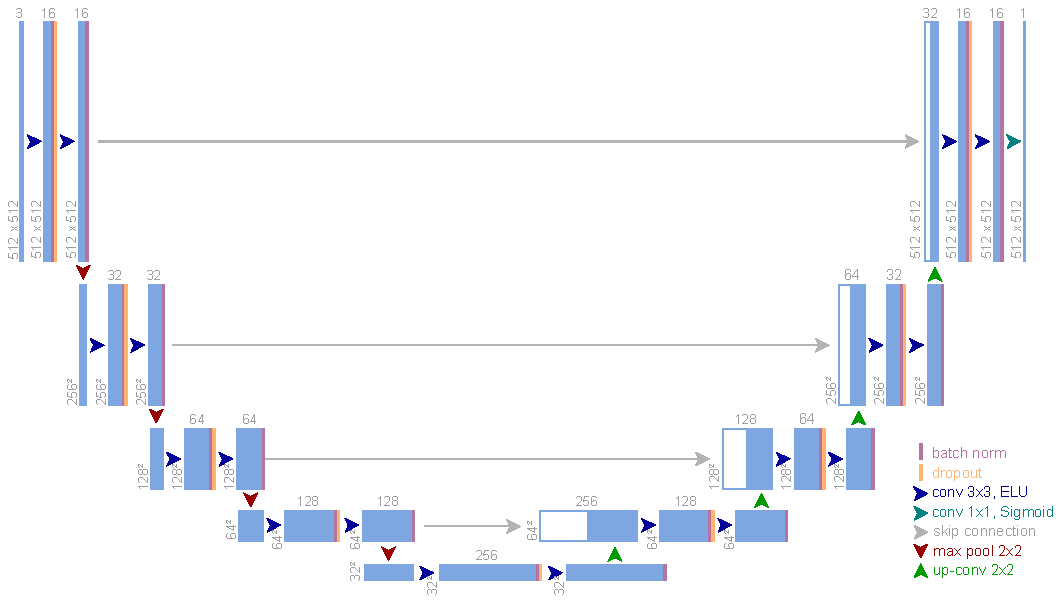
\includegraphics[width=1.\textwidth]{Bilder/own-unet-2mil.pdf} 
	\caption{Bike-U-Net-2 mit 1,946 Mio. Parametern.}
	\label{fig:bike-unet-2}
\end{figure} 


\subsection{Backbone-U-Nets}


\section{Evaluationsmaße}


\section{Hyperparameter}


\section{Pre-Training auf Straßendatensätzen} \label{sec:pre-training-roads}


\section{Testkonzeption}


% \begin{algorithm}
% 	\caption{Algorithmus zum Propagieren und Akkumulieren von Knotenwerten.}\label{lst:prop}
% 	\begin{algorithmic}[1]
% 		\Procedure{Reduce}{$G = (V,E)$} \Comment{$\forall v \in V: value(v) = weight(type(v))$}
% 			\State $sortedNodes \gets topoSort(G)$
% 			\For{$v \in sortedNodes$}\Comment{iteration in topological order}
% 				\If{$v \in R$} 
% 					\State $succ \gets successor(v)$ \Comment{$d^+_G(v) = 1$}
% 					\State $value(succ) \gets value(succ) + value(v)$
% 				\EndIf
% 			\EndFor
% 		\EndProcedure
% 	\end{algorithmic}
% \end{algorithm}

% Nun da alle Knoten die neuen kumulierten Werte haben, lassen sich die reduzierbaren Knoten $r \in R$ entfernen. 

% \mathchardef\mhyphen="2D

% \begin{algorithm}
% 	\caption{Algorithmus zum Kopieren nötiger Kanten von reduzierten Knoten.}\label{lst:reduce}
% 	\begin{algorithmic}[1]
% 		\Procedure{Reduce}{$G = (V,E), C = (F, E_F)$} \Comment{$E_F = \emptyset$}
% 			\State $sortedNodes \gets topoSort(G)$
% 			\For{$v \in sortedNodes$}\Comment{iteration in topological order}
% 				\If{$v \in F$} 
% 					\For{$succ \in successors(v)$}\Comment{$d^+_G(v) \neq 1$}
% 						\If{$succ \in F$}
% 							\State $E_F \gets E_F \cup \{(v, succ)\}$ \Comment{copy $fork \rightarrow fork$}
% 						\EndIf
% 					\EndFor
% 				\Else \Comment{$v \in R$}
% 					\State $succ \gets successor(v)$ \Comment{$d^+_G(v) = 1$}
% 					\For{$pred \in predecessors(v)$}
% 						\If{$pred \in F \land succ \in R$}
% 							\State $E \gets E \cup \{(pred, succ)\}$\Comment{connect $fork \rightarrow non \mhyphen fork$}
% 						\ElsIf {$pred \in F \land succ \in F$}
% 							\State $E_F \gets E_F \cup \{(pred, succ)\}$ \Comment{copy $fork \rightarrow fork$}
% 						\EndIf
% 					\EndFor
% 				\EndIf
% 			\EndFor\label{euclidendwhile}
% 		\EndProcedure
% 	\end{algorithmic}
% \end{algorithm}

% \pagebreak % manueller seitenumbruch

% \section{Gänzliche Einsparung gemeinsamer Teilgraphen} \label{sec:skip_entirely}

% \begin{wrapfigure}{l}{0.35\textwidth}
% 	\centering
% 	\vspace{-30pt} % Manchmal möchte man den oberen Abstand selbst anpassen
% 	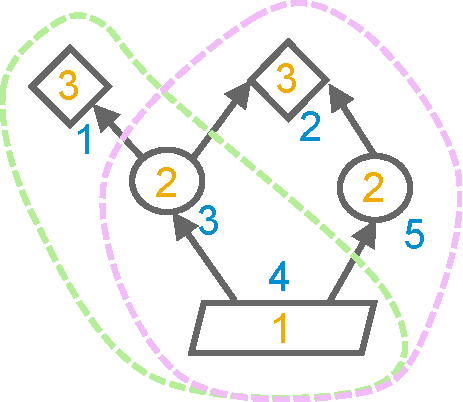
\includegraphics[width=0.30\textwidth]{Bilder/problem_illustration.pdf}
% 	\vspace{-10pt}
% 	% Das folgende ist ein Trick, um "Abbilgung x.y" in eine
% 	% eigene Zeile zu packen. Der Text zwischen [ und ] steht
% 	% im Abbildungsverzeichnis. Der Text darunter wird
% 	% tatsächlich angezeigt.
% 	\caption[Minimalbeispiel zur Teilgraph-Überspringungs-Problematik. Legende wie in \autoref{fig:trans_closures}.]{\unskip}
% 	Minimalbeispiel zur Teilgraph-Überspringungsproblematik. Legende wie in Abb. \ref{fig:trans_closures}.
% 	\label{fig:prob_illu}
% \end{wrapfigure}

% Leider lassen sich bei dem Vergleich zweier Submodelle gemeinsame Teilgraphen nicht gänzlich einsparen, indem der Similarity-Wert über Forks hinaus propagiert wird, um so jedem Knoten im Graph die Summe aller Knotenwerte unter ihm zuzuordnen, da ein gemeinsamer Teilgraph über mehrere Forks betreten werden kann (z.B. der Teilgraph der Schnittmenge von grün und lila in \autoref{fig:trans_closures} kann über Knoten 6 und 5 betreten werden) und nur der maximale Teilgraph gezählt werden darf - ansonsten würde es zu einer doppelten Wertung eines oder mehrerer Knoten kommen. Auch ist die Maximalität  des gemeinsamen Teilgraphen nur mit erheblichen Rechenaufwand, der dem Prinzip des Auslassens entgegensteht, zu überprüfen. Der Graph aus \autoref{fig:prob_illu} ist zur Veranschaulichung geeignet: Es ist schwierig Knoten 4 mit Wert 1 genau einmal zu zählen. Wird Knoten 3 betreten und der restliche Teilgraph (Knoten 4) übersprungen, so wird der Wert 3 zur Similarity addiert.
